% This is the Reed College LaTeX thesis template. Most of the work
% for the document class was done by Sam Noble (SN), as well as this
% template. Later comments etc. by Ben Salzberg (BTS). Additional
% restructuring and APA support by Jess Youngberg (JY).
% Your comments and suggestions are more than welcome; please email
% them to cus@reed.edu
%
% See http://web.reed.edu/cis/help/latex.html for help. There are a
% great bunch of help pages there, with notes on
% getting started, bibtex, etc. Go there and read it if you're not
% already familiar with LaTeX.
%
% Any line that starts with a percent symbol is a comment.
% They won't show up in the document, and are useful for notes
% to yourself and explaining commands.
% Commenting also removes a line from the document;
% very handy for troubleshooting problems. -BTS

% As far as I know, this follows the requirements laid out in
% the 2002-2003 Senior Handbook. Ask a librarian to check the
% document before binding. -SN

%%
%% Preamble
%%
% \documentclass{<something>} must begin each LaTeX document
\documentclass[12pt,twoside]{reedthesis}
% Packages are extensions to the basic LaTeX functions. Whatever you
% want to typeset, there is probably a package out there for it.
% Chemistry (chemtex), screenplays, you name it.
% Check out CTAN to see: http://www.ctan.org/
%%
\usepackage{graphicx,latexsym}
\usepackage{amsmath}
\usepackage{amssymb,amsthm}
\usepackage{longtable,booktabs,setspace}
\usepackage{chemarr} %% Useful for one reaction arrow, useless if you're not a chem major
\usepackage[hyphens]{url}
% Added by CII
\usepackage{hyperref}
\usepackage{lmodern}
\usepackage{float}
\floatplacement{figure}{H}
% End of CII addition
\usepackage{rotating}

% Next line commented out by CII
%%% \usepackage{natbib}
% Comment out the natbib line above and uncomment the following two lines to use the new
% biblatex-chicago style, for Chicago A. Also make some changes at the end where the
% bibliography is included.
%\usepackage{biblatex-chicago}
%\bibliography{thesis}


% Added by CII (Thanks, Hadley!)
% Use ref for internal links
\renewcommand{\hyperref}[2][???]{\autoref{#1}}
\def\chapterautorefname{Chapter}
\def\sectionautorefname{Section}
\def\subsectionautorefname{Subsection}
% End of CII addition

% Added by CII
\usepackage{caption}
\captionsetup{width=5in}
% End of CII addition

% \usepackage{times} % other fonts are available like times, bookman, charter, palatino

% Syntax highlighting #22
  \usepackage{color}
  \usepackage{fancyvrb}
  \newcommand{\VerbBar}{|}
  \newcommand{\VERB}{\Verb[commandchars=\\\{\}]}
  \DefineVerbatimEnvironment{Highlighting}{Verbatim}{commandchars=\\\{\}}
  % Add ',fontsize=\small' for more characters per line
  \usepackage{framed}
  \definecolor{shadecolor}{RGB}{248,248,248}
  \newenvironment{Shaded}{\begin{snugshade}}{\end{snugshade}}
  \newcommand{\AlertTok}[1]{\textcolor[rgb]{0.94,0.16,0.16}{#1}}
  \newcommand{\AnnotationTok}[1]{\textcolor[rgb]{0.56,0.35,0.01}{\textbf{\textit{#1}}}}
  \newcommand{\AttributeTok}[1]{\textcolor[rgb]{0.77,0.63,0.00}{#1}}
  \newcommand{\BaseNTok}[1]{\textcolor[rgb]{0.00,0.00,0.81}{#1}}
  \newcommand{\BuiltInTok}[1]{#1}
  \newcommand{\CharTok}[1]{\textcolor[rgb]{0.31,0.60,0.02}{#1}}
  \newcommand{\CommentTok}[1]{\textcolor[rgb]{0.56,0.35,0.01}{\textit{#1}}}
  \newcommand{\CommentVarTok}[1]{\textcolor[rgb]{0.56,0.35,0.01}{\textbf{\textit{#1}}}}
  \newcommand{\ConstantTok}[1]{\textcolor[rgb]{0.00,0.00,0.00}{#1}}
  \newcommand{\ControlFlowTok}[1]{\textcolor[rgb]{0.13,0.29,0.53}{\textbf{#1}}}
  \newcommand{\DataTypeTok}[1]{\textcolor[rgb]{0.13,0.29,0.53}{#1}}
  \newcommand{\DecValTok}[1]{\textcolor[rgb]{0.00,0.00,0.81}{#1}}
  \newcommand{\DocumentationTok}[1]{\textcolor[rgb]{0.56,0.35,0.01}{\textbf{\textit{#1}}}}
  \newcommand{\ErrorTok}[1]{\textcolor[rgb]{0.64,0.00,0.00}{\textbf{#1}}}
  \newcommand{\ExtensionTok}[1]{#1}
  \newcommand{\FloatTok}[1]{\textcolor[rgb]{0.00,0.00,0.81}{#1}}
  \newcommand{\FunctionTok}[1]{\textcolor[rgb]{0.00,0.00,0.00}{#1}}
  \newcommand{\ImportTok}[1]{#1}
  \newcommand{\InformationTok}[1]{\textcolor[rgb]{0.56,0.35,0.01}{\textbf{\textit{#1}}}}
  \newcommand{\KeywordTok}[1]{\textcolor[rgb]{0.13,0.29,0.53}{\textbf{#1}}}
  \newcommand{\NormalTok}[1]{#1}
  \newcommand{\OperatorTok}[1]{\textcolor[rgb]{0.81,0.36,0.00}{\textbf{#1}}}
  \newcommand{\OtherTok}[1]{\textcolor[rgb]{0.56,0.35,0.01}{#1}}
  \newcommand{\PreprocessorTok}[1]{\textcolor[rgb]{0.56,0.35,0.01}{\textit{#1}}}
  \newcommand{\RegionMarkerTok}[1]{#1}
  \newcommand{\SpecialCharTok}[1]{\textcolor[rgb]{0.00,0.00,0.00}{#1}}
  \newcommand{\SpecialStringTok}[1]{\textcolor[rgb]{0.31,0.60,0.02}{#1}}
  \newcommand{\StringTok}[1]{\textcolor[rgb]{0.31,0.60,0.02}{#1}}
  \newcommand{\VariableTok}[1]{\textcolor[rgb]{0.00,0.00,0.00}{#1}}
  \newcommand{\VerbatimStringTok}[1]{\textcolor[rgb]{0.31,0.60,0.02}{#1}}
  \newcommand{\WarningTok}[1]{\textcolor[rgb]{0.56,0.35,0.01}{\textbf{\textit{#1}}}}

% To pass between YAML and LaTeX the dollar signs are added by CII
\title{MC and GWT}
\author{Your R. Name}
% The month and year that you submit your FINAL draft TO THE LIBRARY (May or December)
\date{May 20xx}
\division{Mathematics and Natural Sciences}
\advisor{Verg}
\institution{Reed College}
\degree{MAI}
%If you have two advisors for some reason, you can use the following
% Uncommented out by CII
% End of CII addition

%%% Remember to use the correct department!
\department{CS}
% if you're writing a thesis in an interdisciplinary major,
% uncomment the line below and change the text as appropriate.
% check the Senior Handbook if unsure.
%\thedivisionof{The Established Interdisciplinary Committee for}
% if you want the approval page to say "Approved for the Committee",
% uncomment the next line
%\approvedforthe{Committee}

% Added by CII
%%% Copied from knitr
%% maxwidth is the original width if it's less than linewidth
%% otherwise use linewidth (to make sure the graphics do not exceed the margin)
\makeatletter
\def\maxwidth{ %
  \ifdim\Gin@nat@width>\linewidth
    \linewidth
  \else
    \Gin@nat@width
  \fi
}
\makeatother

\renewcommand{\contentsname}{Table of Contents}
% End of CII addition

\setlength{\parskip}{0pt}

% Added by CII

\providecommand{\tightlist}{%
  \setlength{\itemsep}{0pt}\setlength{\parskip}{0pt}}

\Acknowledgements{
I want to thank a few people.
}

\Dedication{
You can have a dedication here if you wish.
}

\Preface{
This is an example of a thesis setup to use the reed thesis document class
(for LaTeX) and the R bookdown package, in general.
}

\Abstract{
The preface pretty much says it all.

\par

Second paragraph of abstract starts here.
}

% End of CII addition
%%
%% End Preamble
%%
%
\begin{document}

% Everything below added by CII
  \maketitle

\frontmatter % this stuff will be roman-numbered
\pagestyle{empty} % this removes page numbers from the frontmatter
  \begin{acknowledgements}
    I want to thank a few people.
  \end{acknowledgements}
  \begin{preface}
    This is an example of a thesis setup to use the reed thesis document class
    (for LaTeX) and the R bookdown package, in general.
  \end{preface}
  \hypersetup{linkcolor=black}
  \setcounter{tocdepth}{2}
  \tableofcontents

  \listoftables

  \listoffigures
  \begin{abstract}
    The preface pretty much says it all.
    
    \par
    
    Second paragraph of abstract starts here.
  \end{abstract}
  \begin{dedication}
    You can have a dedication here if you wish.
  \end{dedication}
\mainmatter % here the regular arabic numbering starts
\pagestyle{fancyplain} % turns page numbering back on

\hypertarget{introduction}{%
\chapter*{Introduction}\label{introduction}}
\addcontentsline{toc}{chapter}{Introduction}
\begin{longtable}[]{@{}ll@{}}
\toprule
First Header & Second Header\tabularnewline
\midrule
\endhead
Content Cell & Content Cell\tabularnewline
Content Cell & Content Cell\tabularnewline
\bottomrule
\end{longtable}
Welcome to the \emph{R Markdown} thesis template. This template is based on (and in many places copied directly from) the Reed College LaTeX template, but hopefully it will provide a nicer interface for those that have never used TeX or LaTeX before. Using \emph{R Markdown} will also allow you to easily keep track of your analyses in \textbf{R} chunks of code, with the resulting plots and output included as well. The hope is this \emph{R Markdown} template gets you in the habit of doing reproducible research, which benefits you long-term as a researcher, but also will greatly help anyone that is trying to reproduce or build onto your results down the road.

Hopefully, you won't have much of a learning period to go through and you will reap the benefits of a nicely formatted thesis. The use of LaTeX in combination with \emph{Markdown} is more consistent than the output of a word processor, much less prone to corruption or crashing, and the resulting file is smaller than a Word file. While you may have never had problems using Word in the past, your thesis is likely going to be about twice as large and complex as anything you've written before, taxing Word's capabilities. After working with \emph{Markdown} and \textbf{R} together for a few weeks, we are confident this will be your reporting style of choice going forward.

\textbf{Why use it?}

\emph{R Markdown} creates a simple and straightforward way to interface with the beauty of LaTeX. Packages have been written in \textbf{R} to work directly with LaTeX to produce nicely formatting tables and paragraphs. In addition to creating a user friendly interface to LaTeX, \emph{R Markdown} also allows you to read in your data, to analyze it and to visualize it using \textbf{R} functions, and also to provide the documentation and commentary on the results of your project. Further, it allows for \textbf{R} results to be passed inline to the commentary of your results. You'll see more on this later.

\textbf{Who should use it?}

Anyone who needs to use data analysis, math, tables, a lot of figures, complex cross-references, or who just cares about the final appearance of their document should use \emph{R Markdown}. Of particular use should be anyone in the sciences, but the user-friendly nature of \emph{Markdown} and its ability to keep track of and easily include figures, automatically generate a table of contents, index, references, table of figures, etc. should make it of great benefit to nearly anyone writing a thesis project.

\textbf{For additional help with bookdown}
Please visit \href{https://bookdown.org/yihui/bookdown/}{the free online bookdown reference guide}.

\hypertarget{rmd-basics}{%
\chapter{R Markdown Basics}\label{rmd-basics}}

Here is a brief introduction into using \emph{R Markdown}. \emph{Markdown} is a simple formatting syntax for authoring HTML, PDF, and MS Word documents. \emph{R Markdown} provides the flexibility of \emph{Markdown} with the implementation of \textbf{R} input and output. For more details on using \emph{R Markdown} see \url{http://rmarkdown.rstudio.com}.

Be careful with your spacing in \emph{Markdown} documents. While whitespace largely is ignored, it does at times give \emph{Markdown} signals as to how to proceed. As a habit, try to keep everything left aligned whenever possible, especially as you type a new paragraph. In other words, there is no need to indent basic text in the Rmd document (in fact, it might cause your text to do funny things if you do).

\hypertarget{lists}{%
\section{Lists}\label{lists}}

It's easy to create a list. It can be unordered like
\begin{itemize}
\tightlist
\item
  Item 1
\item
  Item 2
\end{itemize}
or it can be ordered like
\begin{enumerate}
\def\labelenumi{\arabic{enumi}.}
\tightlist
\item
  Item 1
\item
  Item 2
\end{enumerate}
Notice that I intentionally mislabeled Item 2 as number 4. \emph{Markdown} automatically figures this out! You can put any numbers in the list and it will create the list. Check it out below.

To create a sublist, just indent the values a bit (at least four spaces or a tab). (Here's one case where indentation is key!)
\begin{enumerate}
\def\labelenumi{\arabic{enumi}.}
\tightlist
\item
  Item 1
\item
  Item 2
\item
  Item 3
  \begin{itemize}
  \tightlist
  \item
    Item 3a
  \item
    Item 3b
  \end{itemize}
\end{enumerate}
\hypertarget{line-breaks}{%
\section{Line breaks}\label{line-breaks}}

Make sure to add white space between lines if you'd like to start a new paragraph. Look at what happens below in the outputted document if you don't:

Here is the first sentence. Here is another sentence. Here is the last sentence to end the paragraph.
This should be a new paragraph.

\emph{Now for the correct way:}

Here is the first sentence. Here is another sentence. Here is the last sentence to end the paragraph.

This should be a new paragraph.

\hypertarget{r-chunks}{%
\section{R chunks}\label{r-chunks}}

When you click the \textbf{Knit} button above a document will be generated that includes both content as well as the output of any embedded \textbf{R} code chunks within the document. You can embed an \textbf{R} code chunk like this (\texttt{cars} is a built-in \textbf{R} dataset):
\begin{Shaded}
\begin{Highlighting}[]
\KeywordTok{summary}\NormalTok{(cars)}
\end{Highlighting}
\end{Shaded}
\begin{verbatim}
     speed           dist       
 Min.   : 4.0   Min.   :  2.00  
 1st Qu.:12.0   1st Qu.: 26.00  
 Median :15.0   Median : 36.00  
 Mean   :15.4   Mean   : 42.98  
 3rd Qu.:19.0   3rd Qu.: 56.00  
 Max.   :25.0   Max.   :120.00  
\end{verbatim}
\hypertarget{inline-code}{%
\section{Inline code}\label{inline-code}}

If you'd like to put the results of your analysis directly into your discussion, add inline code like this:
\begin{quote}
The \texttt{cos} of \(2 \pi\) is 1.
\end{quote}
Another example would be the direct calculation of the standard deviation:
\begin{quote}
The standard deviation of \texttt{speed} in \texttt{cars} is 5.2876444.
\end{quote}
One last neat feature is the use of the \texttt{ifelse} conditional statement which can be used to output text depending on the result of an \textbf{R} calculation:
\begin{quote}
The standard deviation is less than 6.
\end{quote}
Note the use of \texttt{\textgreater{}} here, which signifies a quotation environment that will be indented.

As you see with \texttt{\$2\ \textbackslash{}pi\$} above, mathematics can be added by surrounding the mathematical text with dollar signs. More examples of this are in \protect\hyperlink{math-sci}{Mathematics and Science} if you uncomment the code in \protect\hyperlink{math}{Math}.

\hypertarget{including-plots}{%
\section{Including plots}\label{including-plots}}

You can also embed plots. For example, here is a way to use the base \textbf{R} graphics package to produce a plot using the built-in \texttt{pressure} dataset:

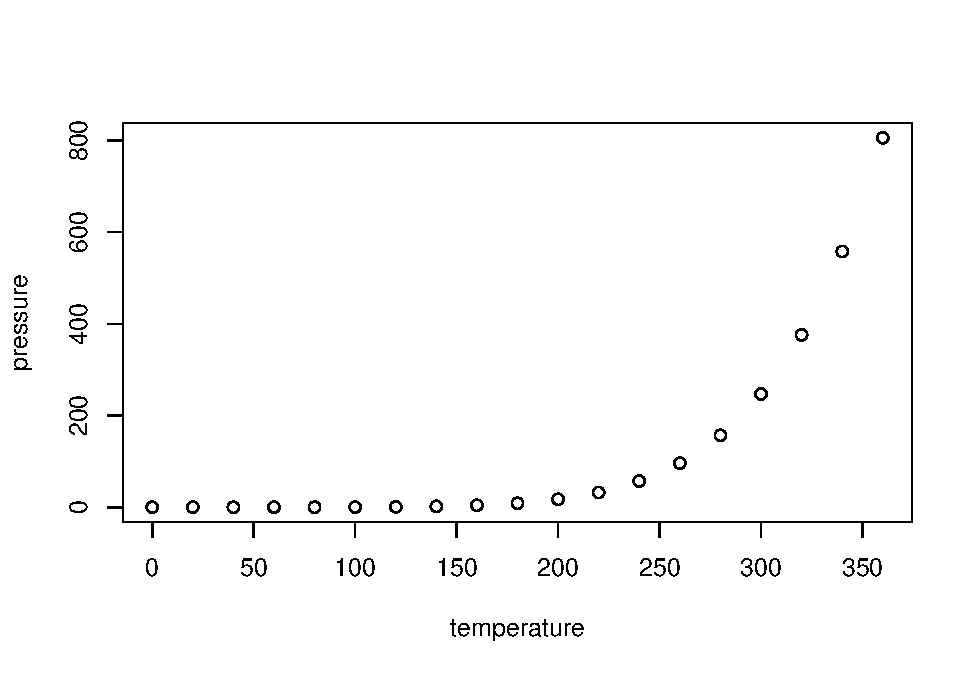
\includegraphics{thesis_files/figure-latex/pressure-1.pdf}

Note that the \texttt{echo=FALSE} parameter was added to the code chunk to prevent printing of the \textbf{R} code that generated the plot. There are plenty of other ways to add chunk options. More information is available at \url{http://yihui.name/knitr/options/}.

Another useful chunk option is the setting of \texttt{cache=TRUE} as you see here. If document rendering becomes time consuming due to long computations or plots that are expensive to generate you can use knitr caching to improve performance. Later in this file, you'll see a way to reference plots created in \textbf{R} or external figures.

\hypertarget{loading-and-exploring-data}{%
\section{Loading and exploring data}\label{loading-and-exploring-data}}

Included in this template is a file called \texttt{flights.csv}. This file includes a subset of the larger dataset of information about all flights that departed from Seattle and Portland in 2014. More information about this dataset and its \textbf{R} package is available at \url{http://github.com/ismayc/pnwflights14}. This subset includes only Portland flights and only rows that were complete with no missing values. Merges were also done with the \texttt{airports} and \texttt{airlines} data sets in the \texttt{pnwflights14} package to get more descriptive airport and airline names.

We can load in this data set using the following command:
\begin{Shaded}
\begin{Highlighting}[]
\NormalTok{flights <-}\StringTok{ }\KeywordTok{read.csv}\NormalTok{(}\StringTok{"data/flights.csv"}\NormalTok{)}
\end{Highlighting}
\end{Shaded}
The data is now stored in the data frame called \texttt{flights} in \textbf{R}. To get a better feel for the variables included in this dataset we can use a variety of functions. Here we can see the dimensions (rows by columns) and also the names of the columns.
\begin{Shaded}
\begin{Highlighting}[]
\KeywordTok{dim}\NormalTok{(flights)}
\end{Highlighting}
\end{Shaded}
\begin{verbatim}
[1] 52808    16
\end{verbatim}
\begin{Shaded}
\begin{Highlighting}[]
\KeywordTok{names}\NormalTok{(flights)}
\end{Highlighting}
\end{Shaded}
\begin{verbatim}
 [1] "month"        "day"          "dep_time"     "dep_delay"   
 [5] "arr_time"     "arr_delay"    "carrier"      "tailnum"     
 [9] "flight"       "dest"         "air_time"     "distance"    
[13] "hour"         "minute"       "carrier_name" "dest_name"   
\end{verbatim}
Another good idea is to take a look at the dataset in table form. With this dataset having more than 50,000 rows, we won't explicitly show the results of the command here. I recommend you enter the command into the Console \textbf{\emph{after}} you have run the \textbf{R} chunks above to load the data into \textbf{R}.
\begin{Shaded}
\begin{Highlighting}[]
\KeywordTok{View}\NormalTok{(flights)}
\end{Highlighting}
\end{Shaded}
While not required, it is highly recommended you use the \texttt{dplyr} package to manipulate and summarize your data set as needed. It uses a syntax that is easy to understand using chaining operations. Below I've created a few examples of using \texttt{dplyr} to get information about the Portland flights in 2014. You will also see the use of the \texttt{ggplot2} package, which produces beautiful, high-quality academic visuals.

We begin by checking to ensure that needed packages are installed and then we load them into our current working environment:
\begin{Shaded}
\begin{Highlighting}[]
\CommentTok{# List of packages required for this analysis}
\NormalTok{pkg <-}\StringTok{ }\KeywordTok{c}\NormalTok{(}\StringTok{"dplyr"}\NormalTok{, }\StringTok{"ggplot2"}\NormalTok{, }\StringTok{"knitr"}\NormalTok{, }\StringTok{"bookdown"}\NormalTok{, }\StringTok{"devtools"}\NormalTok{)}
\CommentTok{# Check if packages are not installed and assign the}
\CommentTok{# names of the packages not installed to the variable new.pkg}
\NormalTok{new.pkg <-}\StringTok{ }\NormalTok{pkg[}\OperatorTok{!}\NormalTok{(pkg }\OperatorTok\StringTok{ }\KeywordTok{installed.packages}\NormalTok{())]}
\CommentTok{# If there are any packages in the list that aren't installed,}
\CommentTok{# install them}
\ControlFlowTok{if}\NormalTok{ (}\KeywordTok{length}\NormalTok{(new.pkg))}
  \KeywordTok{install.packages}\NormalTok{(new.pkg, }\DataTypeTok{repos =} \StringTok{"http://cran.rstudio.com"}\NormalTok{)}
\CommentTok{# Load packages (thesisdown will load all of the packages as well)}
\KeywordTok{library}\NormalTok{(thesisdown)}
\end{Highlighting}
\end{Shaded}
\clearpage

The example we show here does the following:
\begin{itemize}
\item
  Selects only the \texttt{carrier\_name} and \texttt{arr\_delay} from the \texttt{flights} dataset and then assigns this subset to a new variable called \texttt{flights2}.
\item
  Using \texttt{flights2}, we determine the largest arrival delay for each of the carriers.
\end{itemize}
\begin{Shaded}
\begin{Highlighting}[]
\NormalTok{flights2 <-}\StringTok{ }\NormalTok{flights }\OperatorTok\StringTok{ }
\StringTok{  }\KeywordTok{select}\NormalTok{(carrier_name, arr_delay)}
\NormalTok{max_delays <-}\StringTok{ }\NormalTok{flights2 }\OperatorTok\StringTok{ }
\StringTok{  }\KeywordTok{group_by}\NormalTok{(carrier_name) }\OperatorTok
\StringTok{  }\KeywordTok{summarize}\NormalTok{(}\DataTypeTok{max_arr_delay =} \KeywordTok{max}\NormalTok{(arr_delay, }\DataTypeTok{na.rm =} \OtherTok{TRUE}\NormalTok{))}
\end{Highlighting}
\end{Shaded}
A useful function in the \texttt{knitr} package for making nice tables in \emph{R Markdown} is called \texttt{kable}. It is much easier to use than manually entering values into a table by copying and pasting values into Excel or LaTeX. This again goes to show how nice reproducible documents can be! (Note the use of \texttt{results="asis"}, which will produce the table instead of the code to create the table.) The \texttt{caption.short} argument is used to include a shorter title to appear in the List of Tables.
\begin{Shaded}
\begin{Highlighting}[]
\KeywordTok{kable}\NormalTok{(max_delays, }
      \DataTypeTok{col.names =} \KeywordTok{c}\NormalTok{(}\StringTok{"Airline"}\NormalTok{, }\StringTok{"Max Arrival Delay"}\NormalTok{),}
      \DataTypeTok{caption =} \StringTok{"Maximum Delays by Airline"}\NormalTok{,}
      \DataTypeTok{caption.short =} \StringTok{"Max Delays by Airline"}\NormalTok{,}
      \DataTypeTok{longtable =} \OtherTok{TRUE}\NormalTok{,}
      \DataTypeTok{booktabs =} \OtherTok{TRUE}\NormalTok{)}
\end{Highlighting}
\end{Shaded}
\begin{longtable}{lr}
\caption[Max Delays by Airline]{\label{tab:maxdelays}Maximum Delays by Airline}\\
\toprule
Airline & Max Arrival Delay\\
\midrule
Alaska Airlines Inc. & 338\\
American Airlines Inc. & 1539\\
Delta Air Lines Inc. & 651\\
Frontier Airlines Inc. & 575\\
Hawaiian Airlines Inc. & 407\\
\addlinespace
JetBlue Airways & 273\\
SkyWest Airlines Inc. & 421\\
Southwest Airlines Co. & 694\\
United Air Lines Inc. & 472\\
US Airways Inc. & 347\\
\addlinespace
Virgin America & 366\\
\bottomrule
\end{longtable}
The last two options make the table a little easier-to-read.

We can further look into the properties of the largest value here for American Airlines Inc.~To do so, we can isolate the row corresponding to the arrival delay of 1539 minutes for American in our original \texttt{flights} dataset.
\begin{Shaded}
\begin{Highlighting}[]
\NormalTok{flights }\OperatorTok\StringTok{ }\KeywordTok{filter}\NormalTok{(arr_delay }\OperatorTok{==}\StringTok{ }\DecValTok{1539}\NormalTok{, }
\NormalTok{                  carrier_name }\OperatorTok{==}\StringTok{ "American Airlines Inc."}\NormalTok{) }\OperatorTok
\StringTok{  }\KeywordTok{select}\NormalTok{(}\OperatorTok{-}\KeywordTok{c}\NormalTok{(month, day, carrier, dest_name, hour, }
\NormalTok{            minute, carrier_name, arr_delay))}
\end{Highlighting}
\end{Shaded}
\begin{verbatim}
  dep_time dep_delay arr_time tailnum flight dest air_time distance
1     1403      1553     1934  N595AA   1568  DFW      182     1616
\end{verbatim}
We see that the flight occurred on March 3rd and departed a little after 2 PM on its way to Dallas/Fort Worth. Lastly, we show how we can visualize the arrival delay of all departing flights from Portland on March 3rd against time of departure.
\begin{Shaded}
\begin{Highlighting}[]
\NormalTok{flights }\OperatorTok\StringTok{ }\KeywordTok{filter}\NormalTok{(month }\OperatorTok{==}\StringTok{ }\DecValTok{3}\NormalTok{, day }\OperatorTok{==}\StringTok{ }\DecValTok{3}\NormalTok{) }\OperatorTok
\StringTok{  }\KeywordTok{ggplot}\NormalTok{(}\KeywordTok{aes}\NormalTok{(}\DataTypeTok{x =}\NormalTok{ dep_time, }\DataTypeTok{y =}\NormalTok{ arr_delay)) }\OperatorTok{+}\StringTok{ }\KeywordTok{geom_point}\NormalTok{()}
\end{Highlighting}
\end{Shaded}
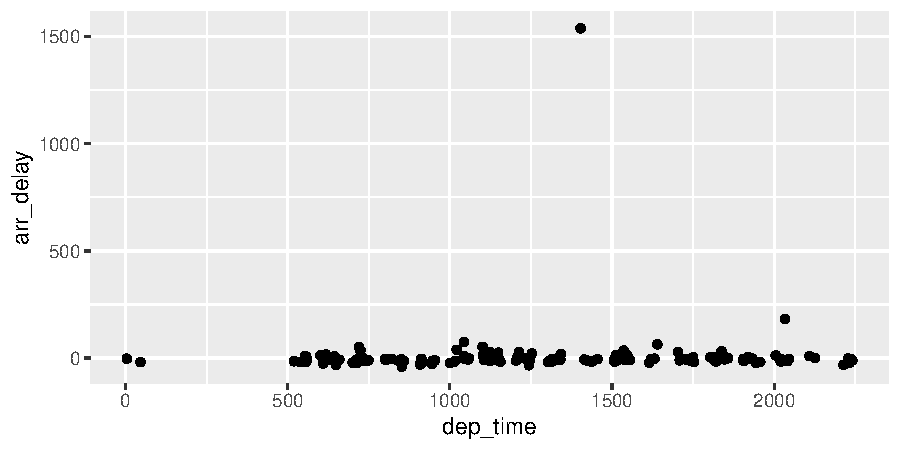
\includegraphics{thesis_files/figure-latex/march3plot-1.pdf}

\hypertarget{additional-resources}{%
\section{Additional resources}\label{additional-resources}}
\begin{itemize}
\item
  \emph{Markdown} Cheatsheet - \url{https://github.com/adam-p/markdown-here/wiki/Markdown-Cheatsheet}
\item
  \emph{R Markdown} Reference Guide - \url{https://www.rstudio.com/wp-content/uploads/2015/03/rmarkdown-reference.pdf}
\item
  Introduction to \texttt{dplyr} - \url{https://cran.rstudio.com/web/packages/dplyr/vignettes/introduction.html}
\item
  \texttt{ggplot2} Documentation - \url{http://docs.ggplot2.org/current/}
\end{itemize}
\hypertarget{math-sci}{%
\chapter{Mathematics and Science}\label{math-sci}}

\hypertarget{math}{%
\section{Math}\label{math}}

\TeX~is the best way to typeset mathematics. Donald Knuth designed \TeX~when he got frustrated at how long it was taking the typesetters to finish his book, which contained a lot of mathematics. One nice feature of \emph{R Markdown} is its ability to read LaTeX code directly.

If you are doing a thesis that will involve lots of math, you will want to read the following section which has been commented out. If you're not going to use math, skip over or delete this next commented section.

\[\sum_{j=1}^n (\delta\theta_j)^2 \leq {{\beta_i^2}\over{\delta_i^2 + \rho_i^2}}
\left[ 2\rho_i^2 + {\delta_i^2\beta_i^2\over{\delta_i^2 + \rho_i^2}} \right] \equiv \omega_i^2
\]

From Informational Dynamics, we have the following (Dave Braden):

After \emph{n} such encounters the posterior density for \(\theta\) is

\[
\pi(\theta|X_1< y_1,\dots,X_n<y_n) \varpropto \pi(\theta) \prod_{i=1}^n\int_{-\infty}^{y_i}
   \exp\left(-{(x-\theta)^2\over{2\sigma^2}}\right)\ dx
\]

Another equation:

\[\det\left|\,\begin{matrix}%
c_0&c_1\hfill&c_2\hfill&\ldots&c_n\hfill\cr
c_1&c_2\hfill&c_3\hfill&\ldots&c_{n+1}\hfill\cr
c_2&c_3\hfill&c_4\hfill&\ldots&c_{n+2}\hfill\cr
\,\vdots\hfill&\,\vdots\hfill&
  \,\vdots\hfill&&\,\vdots\hfill\cr
c_n&c_{n+1}\hfill&c_{n+2}\hfill&\ldots&c_{2n}\hfill\cr
\end{matrix}\right|>0\]
Lapidus and Pindar, Numerical Solution of Partial Differential Equations in Science and
Engineering. Page 54

\[
\int_t\left\{\sum_{j=1}^3 T_j \left({d\phi_j\over dt}+k\phi_j\right)-kT_e\right\}w_i(t)\ dt=0,
   \qquad\quad i=1,2,3.
\]

L\&P Galerkin method weighting functions. Page 55

\[
\sum_{j=1}^3 T_j\int_0^1\left\{{d\phi_j\over dt} + k\phi_j\right\} \phi_i\ dt
   = \int_{0}^1k\,T_e\phi_idt, \qquad i=1,2,3 \]

Another L\&P (p145)

\[
\int_{-1}^1\!\int_{-1}^1\!\int_{-1}^1 f\big(\xi,\eta,\zeta\big)
   = \sum_{k=1}^n\sum_{j=1}^n\sum_{i=1}^n w_i w_j w_k f\big( \xi,\eta,\zeta\big).
\]

Another L\&P (p126)

\[
\int_{A_e} (\,\cdot\,) dx dy = \int_{-1}^1\!\int_{-1}^1 (\,\cdot\,) \det[J] d\xi d\eta.
\]

\hypertarget{chemistry-101-symbols}{%
\section{Chemistry 101: Symbols}\label{chemistry-101-symbols}}

Chemical formulas will look best if they are not italicized. Get around math mode's automatic italicizing in LaTeX by using the argument \texttt{\$\textbackslash{}mathrm\{formula\ here\}\$}, with your formula inside the curly brackets. (Notice the use of the backticks here which enclose text that acts as code.)

So, \(\mathrm{Fe_2^{2+}Cr_2O_4}\) is written \texttt{\$\textbackslash{}mathrm\{Fe\_2\^{}\{2+\}Cr\_2O\_4\}\$}.

\noindent Exponent or Superscript: \(\mathrm{O^-}\)

\noindent Subscript: \(\mathrm{CH_4}\)

To stack numbers or letters as in \(\mathrm{Fe_2^{2+}}\), the subscript is defined first, and then the superscript is defined.

\noindent Bullet: CuCl \(\bullet\) \(\mathrm{7H_{2}O}\)

\noindent Delta: \(\Delta\)

\noindent Reaction Arrows: \(\longrightarrow\) or \(\xrightarrow{solution}\)

\noindent Resonance Arrows: \(\leftrightarrow\)

\noindent Reversible Reaction Arrows: \(\rightleftharpoons\)

\hypertarget{typesetting-reactions}{%
\subsection{Typesetting reactions}\label{typesetting-reactions}}

You may wish to put your reaction in an equation environment, which means that LaTeX will place the reaction where it fits and will number the equations for you.
\begin{equation}
  \mathrm{C_6H_{12}O_6  + 6O_2} \longrightarrow \mathrm{6CO_2 + 6H_2O}
  \label{eq:reaction}
\end{equation}
We can reference this combustion of glucose reaction via Equation \eqref{eq:reaction}.

\hypertarget{other-examples-of-reactions}{%
\subsection{Other examples of reactions}\label{other-examples-of-reactions}}

\(\mathrm{NH_4Cl_{(s)}}\) \(\rightleftharpoons\) \(\mathrm{NH_{3(g)}+HCl_{(g)}}\)

\noindent \(\mathrm{MeCH_2Br + Mg}\) \(\xrightarrow[below]{above}\) \(\mathrm{MeCH_2\bullet Mg \bullet Br}\)

\hypertarget{physics}{%
\section{Physics}\label{physics}}

Many of the symbols you will need can be found on the math page \url{http://web.reed.edu/cis/help/latex/math.html} and the Comprehensive LaTeX Symbol Guide (\url{http://mirror.utexas.edu/ctan/info/symbols/comprehensive/symbols-letter.pdf}).

\hypertarget{biology}{%
\section{Biology}\label{biology}}

You will probably find the resources at \url{http://www.lecb.ncifcrf.gov/~toms/latex.html} helpful, particularly the links to bsts for various journals. You may also be interested in TeXShade for nucleotide typesetting (\url{http://homepages.uni-tuebingen.de/beitz/txe.html}). Be sure to read the proceeding chapter on graphics and tables.

\hypertarget{ch3}{%
\chapter{Neurocognitive Theories of Consciousness}\label{ch3}}

Chapter 1 discussed the philosophical notions of consciousness and introduced the questions engrossed the philosophy of mind. The study of consciousness, however, is a multidisciplinary field of research wherein armchair philosophy fails to iron out all the conundrums singlehandedly; no matter what stance we take towards consciousness (eliminative materialism, substance dualism, or anything in between ), we ultimately need to answer the question of how ``the mental'' interacts with the physical world. The nervous system (more specifically, the brain) is the closest physical entity to the mind. Hence, any account of consciousness must establish (or at least outline) links between the philosophical aspects of consciousness and the neural substrate within (or upon) which it is hosted.

Efforts have been made to bridge between the two disciplines of philosophy (more specifically, what Mandik (2017) calls naturalized philosophy) and neuroscience. Most notably, in her Neurophilosophy, Churchland (1989) attempted to introduce the philosophy of mind to neuroscientists and neuroscience to philosophers (Mandik, 2017). However, most of the contributions to the literature of neurophilosophy are made by philosophers, hence its dominant taste of philosophy. As he notes, neurophilosophy have mainly put three questions in the spotlight: the question of state consciousness (what makes a state conscious?); the question of transitive consciousness (what is the subject of consciousness when one is conscious of it?); and the question of phenomenal character (``when one has a conscious state, in what consists the properties in virtue of which there is something it's like for one to be in that state?'') (Mandik, 2017, p.~460). These questions are referred to as Q\_state, \(Q_{transitive}\), and Q\_\{phenomenal\} in this dissertation, respectively.

It can be noticed that the study of consciousness among scientists lacks the philosophical accuracy exercised by their philosopher peers. In return, the scientific literature on consciousness is more pragmatic and addresses less abstract problems; more specifically, Qstate and Qphenomenal have received the most attention among neuroscientists. The former has mainly been studied in the research into neural correlates of consciousness (NCCs) while the latter has been the subject matter of models of consciousness. This chapter reviews NCC research and two prominent models of consciousness (viz.~the global workspace models and the multiple drafts model). In section 3.2, the global workspace theory of consciousness and its backbone (namely, the global access hypothesis) are reviewed by the relevant body of evidence favoring them. In the same section, Dennett's multiple drafts model is reviewed and compared with the global workspace theory. Finally, in section 3.3, global workspace models are discussed. This chapter is a foundation for Chapter 4, which is about the computational implementations of global workspace models.

\hypertarget{from-neural-correlates-to-models-of-consciousness}{%
\section{From Neural Correlates to Models of Consciousness}\label{from-neural-correlates-to-models-of-consciousness}}

David Chalmers (2010, Chapter 2) has laid down an agenda for the scientific study of consciousness. In his opinion, a scientific account of consciousness needs to, ultimately, relate first-person data of subjective experience to third-person, objective data reflected in observable behaviors or neural processes. He distinguishes six projects for a proper science of consciousness: 1) establishing solid explanations of third-person data; 2) contrasting conscious and unconscious processes; 3) probing the contents of consciousness; 4) finding neural correlates of consciousness; 5) systemizing the connections between first- and third-person data; and 6) inferring fundamental principles of consciousness (2010, pp.~41--47). His proposal mainly concerns answering the descriptive (Why) questions while leaving aside the explanatory (How) and functional (Why) questions. (cf.~Chapter 1).

He, at least implicitly, hopes that having all pieces of the puzzle in place yields an adequate scientific understanding of consciousness; the answers to the How questions, for instance, will be logically entailed if we succeed in stringing the shreds of conscious phenomena (his first five projects) and inferring the constitutional rules of consciousness within this constellation. Some might not find this approach promising---if ever feasible. Nonetheless, it helps us understand why the study of NCCs has become a vital element in the neuroscientific study of consciousness.

NCCs are the neural system(s) or assemblies that can be associated with different aspects of consciousness, e.g., conscious mental states or their contents. This definition posits that NCCs exist somewhere in the brain, and the quest is to find and characterize them. The ultimate goal in the search for NCCs is to use them in the explanations of consciousness, and if that is a viable option, somehow reduce consciousness to its neural correlates. Before doing so, one has to clarify what she means by consciousness, and characterize the association that would count as ``correlation.'' There are several conceptual and methodological obstacles in characterizing NCCs (and making inferences upon them) which are beyond the scope of this chapter (there are entire books on the matter, e.g., Metzinger, 2000). One of the most critical conceptual issues ---after defining what does (and does not) count as correlation--- is that mere correlations can hardly provide any solid explanation of the origins of the association. (Koch, Massimini, Boly, \& Tononi, 2016; Rees \& Frith, 2017).

Neural correlates can be defined in (at least) three different ways, based on the notion of consciousness in question. For state consciousness (NCCstate; in line with Qstate) it can be defined as follows:

A neural system N is an NCC if the state of N correlates directly with states of consciousness. (Chalmers, 2010, p.~61)

On the other hand, NCCs of contents of consciousness (NCCcontent; addressing, loosely speaking, Qtransitive) can be defined as:

A neural correlate of the contents of consciousness is a neural representational system N such that representation of a content in N directly correlates with representation of that content in consciousness. (Chalmers, 2010, p.~65)

It is far trickier to answer Qphenomenal through the study of the neural systems associated with the phenomenal properties of consciousness (NCCphenomenal). An NCCphenomenal can be defined as:

A state N1 of system N is a neural correlate of phenomenal property P if N's being in N1 directly correlates with the subject having P. (Chalmers, 2010, p.~68)

Although NCC research has received much attention, it is crucial to not forget what has made it relevant to consciousness research in the first place: its promise of helping the scientific endeavors in bridging the gap between first- and third-person data. Moreover, it has a (somewhat) strong premise: that the (phenomenal) aspects of consciousness can be reduced to the candidate NCCs. However, it seems NCC research has been more successful in describing the associations between aspects of consciousness and neural phenomena than adequately explaining them. This brings us to models of consciousness, which encompass NCCs within more comprehensive frameworks.

A model of consciousness is a theoretical description of how brain properties relate to phenomenal properties of consciousness using a mechanistic explanation (Seth, 2007; also cf.~Chapter 2). The last part of the definition distinguishes models of consciousness from theories of consciousness that do not necessarily commit to establishing a mechanistic understanding of consciousness (Seth, 2007). The term ``models of consciousness'' has been used slightly differently in the literature of machine consciousness with less commitment to the realization of the model in a neural substrate. For instance, Reggia (2013) deems higher-order thought (HOT) theories (D. Rosenthal, 2005; D. M. Rosenthal, 1996; also cf.~Carruthers, 2016) as models of consciousness since they provide a mechanistic explanation of consciousness and can be realized computationally. Conversely, Seth (2007) opposes HOT theories as such since he believes such mechanistic explanation should be anchored to a neural realization in order to count as a model of consciousness. On the other hand, although Seth (2007) includes Dennett's (1993) multiple drafts model among models of consciousness, it is left out in (Reggia, 2013) as it is not clear how this model can be explicitly implemented computationally.

Among the various models of consciousness (cf.~e.g., Reggia, 2013; Seth, 2007), two are of greater importance for the subject of this thesis: the global workspace models (GWMs), and the multiple draft model (MDM). GWMs are discussed in details in the next section, and MDM will be briefly introduced accordingly.

\hypertarget{global-workspace-theory-of-consciousness}{%
\section{Global Workspace Theory of Consciousness}\label{global-workspace-theory-of-consciousness}}

The global workspace theory (GWT), first presented by Baars (1993) in his magnum opus A Cognitive Theory of Consciousness, initially aimed at contrasting conscious processes from the unconscious ones. It later matured into a comprehensive cognitive theory of consciousness (Baars, 2002) as it received empirical support (Franklin, Strain, Snaider, McCall, \& Faghihi, 2012). It is crucial to note that Baars' original (1993) proposal of GWT is a functional theory of consciousness, yet it became a cornerstone for later models of phenomenal consciousness. The GWT assumes the unconscious (background) processes run in parallel in the distributed system of (specialized) processors and it is the ``coalitions of these processes {[}that{]} enable an agent \ldots{} to make sense of the sensory data coming from the current environmental situation.'' (Franklin, 2011, p.~328). Moreover, since numerous processes are simultaneously running in the brain at any given time, different coalitions emerge in the brain, and, as Franklin (2011) puts it,

{[}These{]} coalitions, incorporating the results of the processing of sensory data, compete for attention in what Baars calls a global workspace. The contents of the winning coalition are broadcast to all other processes. The contents of this broadcast are proposed to be phenomenally conscious. This conscious broadcast serves to recruit other, unconscious, processes to be used to select an action in response to the current situation. GWT is therefore a theory of how consciousness functions within cognition. (p.~328)

In this theory, the global workspace (GW) acts both as a ``bottleneck'' of information and a broadcaster. Figure 3.1 (Franklin et al., 2012, fig.~1) roughly shows how GW filters the competing information ``produced'' by different sensory coalitions and broadcasts to other areas. It can be generalized to other processes as well. See Figure 3.2 (Shanahan, 2010, fig.~4.1). Before discussing the details of how GWT is realized in the brain, we need to discuss the theoretical and empirical foundations of GWT, to which subsections 3.2.1 and 3.2.2 are dedicated.

\hypertarget{the-conscious-limitedness-and-the-unconscious-immenseness}{%
\subsection{The Conscious Limitedness and The Unconscious Immenseness}\label{the-conscious-limitedness-and-the-unconscious-immenseness}}

The point of departure for GWT is the well-established finding that limited conscious capacity of the brain (e.g., in coherent binding of sensory inputs, conscious access to memory, and cognitively demanding tasks) coexists along with many unconscious, parallel processes (such as coordination of body movements and maintaining balance, or perception of volumes in vision) happening within a ``massive beehive of neural assemblies, cells, layers, and connections, each flexibly specialized in some set of tasks.'' (Baars, 2017, pp.~232--233). The limited conscious capacity has been known to philosophers, psychologists, and cognitive (neuro)scientists for decades. For a detailed review of limited capacity in attention, action, memory, and vision, see (Baars, 1993, secs. 1.3.3-1.3.6). Baars also reviews the consensus around unconscious parallel processes in the brain and discusses their properties (1993, sec.~1.4). For a more concise review, see (Baars, 1997b). GWT suggests the global access hypothesis (GAH) can explain how these different kinds of processes coexist---and interact. Here, two of the most intuitive psychological bodies of evidence for parallel processes are reviewed: the mental lexical access, and the autobiographical memory.

It is estimated that an average 20-year-old native English speaker knows roughly 42,000 unique lemmas (Brysbaert, Stevens, Mandera, \& Keuleers, 2016). Many of these lemmas are shared by different words, meaning that the native speaker's lexicon is far more abundant. Moreover, many words with the same morphology differ remarkably in their meanings. It is evident that one does not (and, in fact, cannot) consciously retrieve meanings of every word from her lexicon to comprehend sentences in the everyday use of language. Additionally, there is compelling evidence that the semantic context of words is autonomously (and unconsciously) processed before the correct connotation of the word is (consciously) comprehended. (Swinney, 1979; as cited in Baars, 1993). Baars elaborates on this with an example:

A typical experiment in this literature has the following format: Subjects listen to a sentence fragment ending in an ambiguous word, such as ``They all rose \ldots{}'' The word ``rose'' can be either a verb or a noun, but in this sentence context it must be a verb. How long will it take for this fact to influence the interpretation of the next word? To test this, one of two words is presented, either flower, or stood. Subjects are asked to decide quickly whether the presented word is a real English word or not. If the subjects make use of the sentence context in their lexical decision task, the verb ``rose'' should speed decisions for ``stood,'' because the two words are similar in meaning and syntax; if the context is not used, there should be no time difference between the verb ``stood'' and the noun ``flower.'' Several investigators have found that for the first few hundred milliseconds, the sentence context has no influence at all \ldots{} Thus it seems as if lexical access is autonomous and context-free for a few hundred milliseconds. After this period, prior context does influence the choice of interpretation. (Baars, 1993, p.~46)

More recent research has focused on characterizing the neural processes that give rise to this phenomenon (for recent studies on semantic priming, cf., e.g., Fahimi Hnazaee, Khachatryan, \& Van Hulle, 2018; Lerner, Bentin, \& Shriki, 2012).

Another interesting phenomenon is the quick accessibility of individual memories within the autobiographical memory. In his classic study, Standing (1973) reports that, under certain measurement conditions, subjects are capable of distinguishing as many as 10,000 images previously seen only for a few seconds each. Based on these findings, Baars writes:

We can get an everyday sense of this remarkable memory performance from the common experience of recognizing a film seen only once, many years ago, with a sudden sense of familiarity. Often we can even predict the next scene. It seems that the brain creates memories of the stream of experience merely by paying attention to it; but humans are always paying attention to new and interesting things, suggesting that our spontaneous autobiographical memory must be very large indeed. Once again we have a vast unconscious domain, and we gain access to it using conscious thought. Mere consciousness of an event helps to store it in memory, and when we experience it again we can voluntarily recognize one distinctive episode from many millions in memory. (2017, p.~234)

\hypertarget{the-global-access-hypothesis}{%
\subsection{The Global Access Hypothesis}\label{the-global-access-hypothesis}}

GWT introduces GAH using the classic theater metaphor of consciousness (Baars, 1997a). In this metaphor, the parallel processes compete in order to take over the stage, and the contents of the winner become accessible (or, is ``broadcast'') to other processes. The working memory is also on the stage; it can be seen as either as a computational resource ``within'' the GW, available to the winning process, or as a ``medium'' hosting the information contents of the processes . The content appearing on the stage is experienced consciously by the subject when illuminated by the spotlight fo attention.

Figure 3.3 (adapted from Baars, 2017, fig.~16.1) shows a schematic view of GAH and the stage, the spotlight, and the processes accessing the GW. These processes, both the competitors and the audience ---although most of them can undertake both roles--- are not limited to sensory inputs and verbal and non-verbal outputs; they can also be related to perceptual and cognitive contexts (examples of the latter are intentions, expectations, and the ``self'') or the unconscious resources (such as interpretations, memories, language, and automatism).

GAH has received a staggering amount of converging empirical and philosophical support (cf., e.g., Cooney \& Gazzaniga, 2003; Dehaene, Kerszberg, \& Changeux, 2001; Dehaene, Sergent, \& Changeux, 2003; D. Dennett, 2001; Freeman, 2003; as cited in Baars, 2017). Although there are discrepancies in characterization and properties of the ``GW'' in these theories, there is a decent consensus among scholars around GAH, especially with formalizations close to that of GWT---and such consensuses are quite scarce in the field of consciousness studies. A more detailed review of the literature (from 1983 to 2001) supporting GAH can be found in (Baars, 2002). Before moving on to GWMs (which are realizations of GWT) let us address Daniel Dennett's multiple drafts model as it gives additional insights into the GAH.

\hypertarget{multiple-drafts-model}{%
\subsection{Multiple Drafts Model}\label{multiple-drafts-model}}

Daniel Dennett's MDM (1993; 2001) belongs to (and stands out as an exemplary member of) the family of narrative interpretive theories of consciousness. It was developed as an alternative to the metaphor of ``Cartesian Theater'' which posits that consciousness is a result of the consolidation of information at some spatial or functional location or in a special mode or format wherein they become accessible to the ``self.'' (Van Gulick, 2018, sec.~9.4). Discussion of Descartes' dualist theory of mind is well beyond this manuscript, but the keen reader can consult (Hatfield, 2018, sec.~3.4; Robinson, 2017, sec.~1.2; Van Gulick, 2018, secs. 4.5, 8.1).

The MDM borrows ``elements of both representationalism and higher-order theory but does so in a way that varies interestingly from the more standard versions of either providing a more interpretational and less strongly realist view of consciousness.'' (Van Gulick, 2018, sec.~9.4, par. 1). The multiple pieces of information made by brain regions are considered ``drafts''; passed from one region to another and subject to constant modification as they travel around. Drafts gain ``fame'' in the brain based on the degree to which they engage the processors. The drafts compete to gain more fame, and content of the most famous draft becomes ``conscious.'' According to MDM, qualia are not phenomena that need explanations but mere epiphenomena of gaining the most fame, hence it is an eliminativists theory of consciousness (Ramsey, 2019, sec.~3.3). This implies that many of the questions mentioned in Chapter 1 are irrelevant---what does it mean to explain something that does not ``exist''? MDM also explains the self as a ``center of narrative gravity'' (D. Dennett, 1992). As Van Gulick (2018) writes,

The MDM treats the self as an emergent or virtual aspect of the coherent roughly serially narrative that is constructed through the interactive play of contents in the system. Many of those contents are bound together at the intentional level as perceptions or fixations from a relatively unified and temporally extended point of view, i.e., they cohere in their contents as if they were the experiences of {[}an{]} ongoing self. But it is the order of dependence that is crucial to the MDM account. The relevant contents are not unified because they are all observed by a single self, but just the converse. It is because they are unified and coherent at the level of content that they count as the experiences of a single self, at least of a single virtual self. (sec.~9.4, para. 3)

The MDM has been extremely controversial yet amazingly influential. One of the most important criticisms against MDM (and more specifically, the way Dennett sells it in his seminal book Consciousness Explained (1993)) is that it, although built upon empirical evidence, fails to provide a realist, scientifically testable model for consciousness (see, e.g., McGinn, 1995). The keen reader will gain insights into the critiques of the MDM in the peer commentary of Dennett and Kinsbourne's (1992) paper.

The MDM and the GWT both endorse the GAH, but in different ways. The MDM is in line with the GAH, as it emphasizes on the accessibility of the drafts to the processors, but does not set forth any locus where they consolidate---more precisely, it explicitly denies that. The GWT, on the other hand, limits the global accessibility to the content reaching the stage of the GW, while there is no stage in the MDM metaphor. The GWT --even its original version where it has no commitment to any physical realization, see next subsection--- is more ``scientific'' for at least three reasons: it can be formally defined, beyond metaphorical interpretations; it gives a mechanistic explanation for consciousness; and, most importantly, it makes specific predictions that can be verified scientifically. The GWMs are even more powerful compared to the basic GWT for they discuss realization of the GW, and, one way or another, anchor themselves to the underlying neurobiology and neuroanatomy of the brain. These realizations are discussed in the next section.

\hypertarget{global-workspace-models-the-realizations-of-the-gwt}{%
\section{Global Workspace Models: The Realizations of the GWT}\label{global-workspace-models-the-realizations-of-the-gwt}}

As mentioned earlier in this chapter, Baars' (1993) basic GWT is a functional theory of conscious experience---it does not commit to any (specific) realization. This basic theory makes six theoretical predictions, as mentioned in (Baars, 2017, table 16.1). Based upon it, he proposed seven models with increasingly wider scopes of empirical predictions (for a short overview, see Baars, 2017, table 16.2). Although these models are in accord with specific empirical evidence from the neuroscientific study of consciousness, they are not specifically (or visibly enough) linked to plausible neuroanatomical realizations.

Further research tried to bridge the gap between the mental and realization levels of the mechanistic explanation of consciousness. For a comprehensive review, see (Baars, 2002). Among the GWMs studied in the literature, Shanahan's (2010) dynamic version of a GWM (denoted as DGWM from now on) deserves more attention as it tries to incorporate embodiment within a GW framework. This model roots in his earlier architecture (Shanahan, 2006) that explicitly included the internal stimuli in a GWM. In the remainder of this chapter, the DGWM is discussed.

Shanahan augments an intermediate level of abstraction, namely neural dynamics (ND), between the TLM's two lowest levels of analysis (viz., Lmental and Lrealization; see Chapter 2). Consequently, DGWN puts forth an explication for the (possible) structure of the GW, and an explanation for how this structure serves as a GW. Haikonen (2011) compares various aspects of Baars GWMs to Shanahan's DGWM. Perhaps one of the most important differences between them is that Shanahan emphasizes that GW is an infrastructure of information exchange (wherein competition takes place as well). Hence it is substantially different from Baars' working memory account. Haikonen elaborates on this distinction:

Shanahan's view about the global workspace is different. Firstly, he wishes to distance himself from the theater model by recasting the role of the global workspace. Instead of a working memory, the global workspace should be thought as a communications infrastructure that connects the various autonomous units with each other: ``Indeed, unless recast this way, the putative workspace might be mistaken for a dedicated brain region, something akin to the Cartesian theater ridiculed by Dennett, {[}a place in the brain where `it all comes together and consciousness happens.'{]}'' {[}(Shanahan, 2010, p.~111){]} Shanahan proposes that in the brain, the global workspace consists of the white matter connective core that connects the various brain areas with each other. But this infrastructure is not to be taken only as a transmission medium. According to Shanahan: ``GWS is not only the locus of broadcast, but also the arena for competition between rival coalitions and the medium of coupling for the members of those coalitions.'' {[}(Shanahan, 2010, p.~147){]} This infrastructure has limited capacity and therefore forms a temporally limiting bottleneck; this would explain the serial nature of consciousness. (Haikonen, 2011, pp.~339--340)

Shanahan uses graph theory to characterize possible structures that can be plausible candidates for a putative GW. He seeks a network structure that has two properties: it has specialized autonomous modules, and the modules are efficiently interconnected. Such networks are called small-world structures (SWS) as they share similar mathematical properties with other networks found in the wild . SWSs entered the scientific discourse after Watts and Strogatz (1998) introduced a rewiring algorithm that recursively optimizes the structural properties of a regular graph to show properties of SWSs . SWSs has been studied widely since, and a rich literature asserts that brain networks have small-world properties (SWPs; Bassett \& Bullmore, 2006; Sporns \& Zwi, 2004; for a more systematic introduction, consult Sporns, 2010, Chapters 3--4). Several rewiring algorithms have been proposed that resemble the natural development of the human brain and can generate SWSs (e.g., see Jarman, Steur, Trengove, Tyukin, \& Leeuwen, 2017).

Shanahan (2010, Chapter 4) explains how the coalition can lead to a GW-like structure suitable for broadcast if information. To do so, he takes two steps. First, he investigates formal representations of graphs have the desired structure. He starts with the classic Watts and Strogatz network and suggests an adapted graph wherein highly intraconnected ``communities'' enhance the modularity of the network (pp.~119-121). He then distinguishes ``connector hubs,'' i.e., the nodes that with ``high trans-modular connectivity,'' and names the links between such hubs the ``connective core'' (pp.~121-122). Finally, he suggests that the communities themselves can be thought of as smaller SWSs. Hence, he generalizes the network into a ``scale-free,'' hierarchical structure, wherein modularity and SWPs are present at different levels of organization---locally and globally (p.~122). These models are shown in Figure 3.4 (adapted from Shanahan, 2010, figs. 4.6-4.8).

In the second step, he proposes candidate neuroanatomical structures for a presumed GW. More specifically, he suggests the long-range white matter tracts (connecting distant regions of the cortex) as a likely substrate for GW, and the ``thalamocortical pathways {[}that{]} relay traffic to and from different parts of the cortex, and may also play a role in the putative workspace'' (pp.~125-126). Then, he shows that applying the hierarchical SWS introduced in the first step to structural parcellation of the cortex into highly intraconnected brain regions (as in, e.g., Hagmann et al., 2008) yields a similar network structure (p.~126). Finally, he distinguishes a ``connective core'' within the anatomical network and concludes that it is indeed the possible locus for a neural GW in the brain. This proposal is backed by neuroanatomical findings and mathematical modeling of such network structures, and most importantly, the connective core is capable of manifesting the principal properties of a GW (see Figure 3.1). Shanahan writes,

The connective core of a hierarchically modular network is topologically well placed to realize both broadcast (because influence funnels into and fans out from the centre) and competition (because it acts as a limited capacity bottleneck). So it is an ideal candidate for the anatomical locus of a global workspace. (2010, fig.~4.11 caption)

These models are depicted in Figure 3.5 (adapted from Shanahan, 2010, figs. 4.9-4.11).

Shanahan's DGWM is of the highest value among GWMs for two main reasons. Firstly, it has more explanatory power compared to its predecessors; e.g., it explains embodiment and explicates the inner narrative property of consciousness. Secondly, and most importantly, it is decently anchored to the neural substrate via the intermediate level of abstraction it places between Lmental and Lrealization. The latter point has a remarkable implication: it guarantees a mechanical link between those levels of analysis, hence partitioning the arduous enigma of answering the How questions into two smaller, more feasible problems: explanations at Lmental, and explications of (structural) realization of the GW in the Lrealization. Based upon this, Chapter 4 probes computational implementations of GWMs, and gives a review (and applies) a benchmark to roughly assess the resemblance of such models to human consciousness.

Figure 1 GW as a bottleneck and as a broadcaster (adapted from Franklin et al., 2012, fig.~1)

Figure 2 GW architecture (adapted from Shanahan, 2010, fig.~4.1)

Figure 3 A schematic diagram of global access. A schematic diagram of global access (adapted from Baars, 2017, fig.~16.1)

\hypertarget{ref-labels}{%
\chapter{Tables, Graphics, References, and Labels}\label{ref-labels}}

\hypertarget{tables}{%
\section{Tables}\label{tables}}

In addition to the tables that can be automatically generated from a data frame in \textbf{R} that you saw in \protect\hyperlink{rmd-basics}{R Markdown Basics} using the \texttt{kable} function, you can also create tables using \emph{pandoc}. (More information is available at \url{http://pandoc.org/README.html\#tables}.) This might be useful if you don't have values specifically stored in \textbf{R}, but you'd like to display them in table form. Below is an example. Pay careful attention to the alignment in the table and hyphens to create the rows and columns.
\begin{longtable}[]{@{}ccc@{}}
\caption{\label{tab:inher} Correlation of Inheritance Factors for Parents and Child}\tabularnewline
\toprule
\begin{minipage}[b]{0.29\columnwidth}\centering
Factors\strut
\end{minipage} & \begin{minipage}[b]{0.46\columnwidth}\centering
Correlation between Parents \& Child\strut
\end{minipage} & \begin{minipage}[b]{0.16\columnwidth}\centering
Inherited\strut
\end{minipage}\tabularnewline
\midrule
\endfirsthead
\toprule
\begin{minipage}[b]{0.29\columnwidth}\centering
Factors\strut
\end{minipage} & \begin{minipage}[b]{0.46\columnwidth}\centering
Correlation between Parents \& Child\strut
\end{minipage} & \begin{minipage}[b]{0.16\columnwidth}\centering
Inherited\strut
\end{minipage}\tabularnewline
\midrule
\endhead
\begin{minipage}[t]{0.29\columnwidth}\centering
Education\strut
\end{minipage} & \begin{minipage}[t]{0.46\columnwidth}\centering
-0.49\strut
\end{minipage} & \begin{minipage}[t]{0.16\columnwidth}\centering
Yes\strut
\end{minipage}\tabularnewline
\begin{minipage}[t]{0.29\columnwidth}\centering
Socio-Economic Status\strut
\end{minipage} & \begin{minipage}[t]{0.46\columnwidth}\centering
0.28\strut
\end{minipage} & \begin{minipage}[t]{0.16\columnwidth}\centering
Slight\strut
\end{minipage}\tabularnewline
\begin{minipage}[t]{0.29\columnwidth}\centering
Income\strut
\end{minipage} & \begin{minipage}[t]{0.46\columnwidth}\centering
0.08\strut
\end{minipage} & \begin{minipage}[t]{0.16\columnwidth}\centering
No\strut
\end{minipage}\tabularnewline
\begin{minipage}[t]{0.29\columnwidth}\centering
Family Size\strut
\end{minipage} & \begin{minipage}[t]{0.46\columnwidth}\centering
0.18\strut
\end{minipage} & \begin{minipage}[t]{0.16\columnwidth}\centering
Slight\strut
\end{minipage}\tabularnewline
\begin{minipage}[t]{0.29\columnwidth}\centering
Occupational Prestige\strut
\end{minipage} & \begin{minipage}[t]{0.46\columnwidth}\centering
0.21\strut
\end{minipage} & \begin{minipage}[t]{0.16\columnwidth}\centering
Slight\strut
\end{minipage}\tabularnewline
\bottomrule
\end{longtable}
We can also create a link to the table by doing the following: Table \ref{tab:inher}. If you go back to \protect\hyperlink{loading-and-exploring-data}{Loading and exploring data} and look at the \texttt{kable} table, we can create a reference to this max delays table too: Table \ref{tab:maxdelays}. The addition of the \texttt{(\textbackslash{}\#tab:inher)} option to the end of the table caption allows us to then make a reference to Table \texttt{\textbackslash{}@ref(tab:label)}. Note that this reference could appear anywhere throughout the document after the table has appeared.

\clearpage

\hypertarget{figures}{%
\section{Figures}\label{figures}}

If your thesis has a lot of figures, \emph{R Markdown} might behave better for you than that other word processor. One perk is that it will automatically number the figures accordingly in each chapter. You'll also be able to create a label for each figure, add a caption, and then reference the figure in a way similar to what we saw with tables earlier. If you label your figures, you can move the figures around and \emph{R Markdown} will automatically adjust the numbering for you. No need for you to remember! So that you don't have to get too far into LaTeX to do this, a couple \textbf{R} functions have been created for you to assist. You'll see their use below.

In the \textbf{R} chunk below, we will load in a picture stored as \texttt{reed.jpg} in our main directory. We then give it the caption of ``Reed logo'', the label of ``reedlogo'', and specify that this is a figure. Make note of the different \textbf{R} chunk options that are given in the R Markdown file (not shown in the knitted document).
\begin{Shaded}
\begin{Highlighting}[]
\KeywordTok{include_graphics}\NormalTok{(}\DataTypeTok{path =} \StringTok{"figure/reed.jpg"}\NormalTok{)}
\end{Highlighting}
\end{Shaded}
\begin{figure}

\includegraphics[width=3.47in]{figure/reed} \caption{Reed logo}\label{fig:reedlogo}
\end{figure}
Here is a reference to the Reed logo: Figure \ref{fig:reedlogo}. Note the use of the \texttt{fig:} code here. By naming the \textbf{R} chunk that contains the figure, we can then reference that figure later as done in the first sentence here. We can also specify the caption for the figure via the R chunk option \texttt{fig.cap}.

\clearpage

Below we will investigate how to save the output of an \textbf{R} plot and label it in a way similar to that done above. Recall the \texttt{flights} dataset from Chapter \ref{rmd-basics}. (Note that we've shown a different way to reference a section or chapter here.) We will next explore a bar graph with the mean flight departure delays by airline from Portland for 2014. Note also the use of the \texttt{scale} parameter which is discussed on the next page.
\begin{Shaded}
\begin{Highlighting}[]
\NormalTok{flights }\OperatorTok\StringTok{ }\KeywordTok{group_by}\NormalTok{(carrier) }\OperatorTok
\StringTok{  }\KeywordTok{summarize}\NormalTok{(}\DataTypeTok{mean_dep_delay =} \KeywordTok{mean}\NormalTok{(dep_delay)) }\OperatorTok
\StringTok{  }\KeywordTok{ggplot}\NormalTok{(}\KeywordTok{aes}\NormalTok{(}\DataTypeTok{x =}\NormalTok{ carrier, }\DataTypeTok{y =}\NormalTok{ mean_dep_delay)) }\OperatorTok{+}
\StringTok{  }\KeywordTok{geom_bar}\NormalTok{(}\DataTypeTok{position =} \StringTok{"identity"}\NormalTok{, }\DataTypeTok{stat =} \StringTok{"identity"}\NormalTok{, }\DataTypeTok{fill =} \StringTok{"red"}\NormalTok{)}
\end{Highlighting}
\end{Shaded}
\begin{figure}
\centering
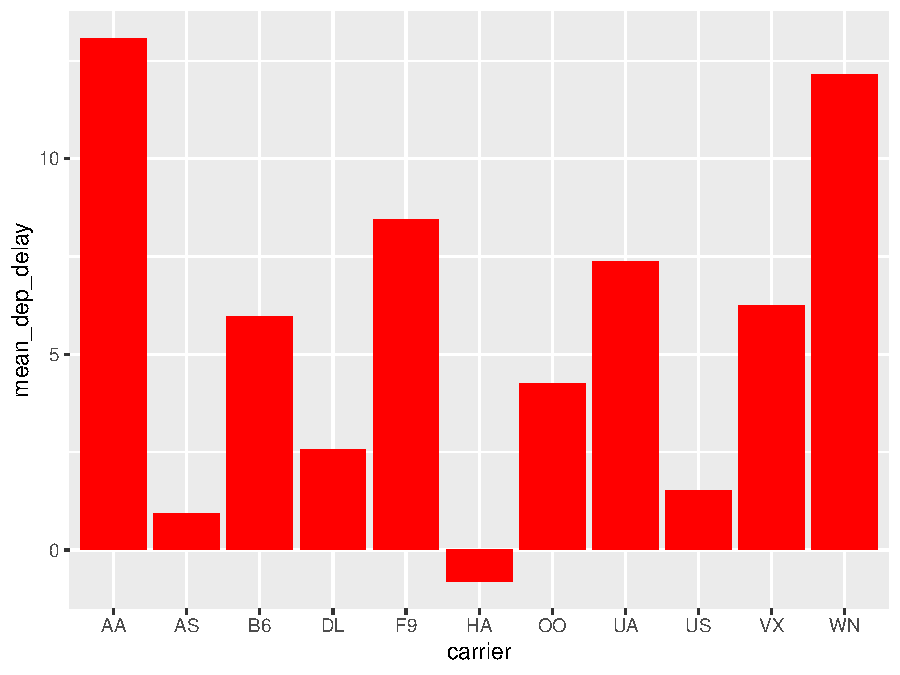
\includegraphics{thesis_files/figure-latex/delaysboxplot-1.pdf}
\caption{\label{fig:delaysboxplot}Mean Delays by Airline}
\end{figure}
Here is a reference to this image: Figure \ref{fig:delaysboxplot}.

A table linking these carrier codes to airline names is available at \url{https://github.com/ismayc/pnwflights14/blob/master/data/airlines.csv}.

\clearpage

Next, we will explore the use of the \texttt{out.extra} chunk option, which can be used to shrink or expand an image loaded from a file by specifying \texttt{"scale=\ "}. Here we use the mathematical graph stored in the ``subdivision.pdf'' file.
\begin{figure}
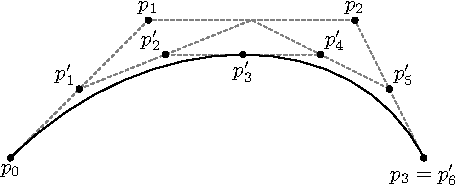
\includegraphics[scale=0.75]{figure/subdivision} \caption{Subdiv. graph}\label{fig:subd}
\end{figure}
Here is a reference to this image: Figure \ref{fig:subd}. Note that \texttt{echo=FALSE} is specified so that the \textbf{R} code is hidden in the document.

\textbf{More Figure Stuff}

Lastly, we will explore how to rotate and enlarge figures using the \texttt{out.extra} chunk option. (Currently this only works in the PDF version of the book.)
\begin{figure}
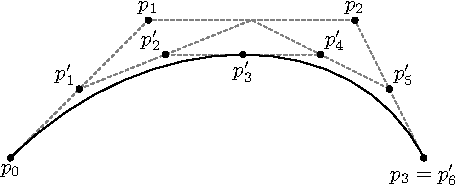
\includegraphics[angle=180, scale=1.1]{figure/subdivision} \caption{A Larger Figure, Flipped Upside Down}\label{fig:subd2}
\end{figure}
As another example, here is a reference: Figure \ref{fig:subd2}.

\hypertarget{footnotes-and-endnotes}{%
\section{Footnotes and Endnotes}\label{footnotes-and-endnotes}}

You might want to footnote something.\footnote{footnote text} The footnote will be in a smaller font and placed appropriately. Endnotes work in much the same way. More information can be found about both on the CUS site or feel free to reach out to \href{mailto:data@reed.edu}{\nolinkurl{data@reed.edu}}.

\hypertarget{bibliographies}{%
\section{Bibliographies}\label{bibliographies}}

Of course you will need to cite things, and you will probably accumulate an armful of sources. There are a variety of tools available for creating a bibliography database (stored with the .bib extension). In addition to BibTeX suggested below, you may want to consider using the free and easy-to-use tool called Zotero. The Reed librarians have created Zotero documentation at \url{http://libguides.reed.edu/citation/zotero}. In addition, a tutorial is available from Middlebury College at \url{http://sites.middlebury.edu/zoteromiddlebury/}.

\emph{R Markdown} uses \emph{pandoc} (\url{http://pandoc.org/}) to build its bibliographies. One nice caveat of this is that you won't have to do a second compile to load in references as standard LaTeX requires. To cite references in your thesis (after creating your bibliography database), place the reference name inside square brackets and precede it by the ``at'' symbol. For example, here's a reference to a book about worrying: \texttt{@key} is Depp, Torous, \& Thompson (\protect\hyperlink{ref-Molina1994}{1994}) and \texttt{{[}@key{]}} is (Depp et al., \protect\hyperlink{ref-Molina1994}{1994}; Noble, \protect\hyperlink{ref-noble2002}{2002}; \protect\hyperlink{ref-reedweb2007}{2007}, p. 85). This \texttt{Molina1994} entry appears in a file called \texttt{thesis.bib} in the \texttt{bib} folder. This bibliography database file was created by a program called BibTeX. You can call this file something else if you like (look at the YAML header in the main .Rmd file) and, by default, is to placed in the \texttt{bib} folder.

For more information about BibTeX and bibliographies, see our CUS site (\url{http://web.reed.edu/cis/help/latex/index.html})\footnote{Reed~College (\protect\hyperlink{ref-reedweb2007}{2007})}. There are three pages on this topic: \emph{bibtex} (which talks about using BibTeX, at \url{http://web.reed.edu/cis/help/latex/bibtex.html}), \emph{bibtexstyles} (about how to find and use the bibliography style that best suits your needs, at \url{http://web.reed.edu/cis/help/latex/bibtexstyles.html}) and \emph{bibman} (which covers how to make and maintain a bibliography by hand, without BibTeX, at \url{http://web.reed.edu/cis/help/latex/bibman.html}). The last page will not be useful unless you have only a few sources.

If you look at the YAML header at the top of the main .Rmd file you can see that we can specify the style of the bibliography by referencing the appropriate csl file. You can download a variety of different style files at \url{https://www.zotero.org/styles}. Make sure to download the file into the csl folder.

\textbf{Tips for Bibliographies}
\begin{itemize}
\tightlist
\item
  Like with thesis formatting, the sooner you start compiling your bibliography for something as large as thesis, the better. Typing in source after source is mind-numbing enough; do you really want to do it for hours on end in late April? Think of it as procrastination.
\item
  The cite key (a citation's label) needs to be unique from the other entries.
\item
  When you have more than one author or editor, you need to separate each author's name by the word ``and'' e.g.~\texttt{Author\ =\ \{Noble,\ Sam\ and\ Youngberg,\ Jessica\},}.
\item
  Bibliographies made using BibTeX (whether manually or using a manager) accept LaTeX markup, so you can italicize and add symbols as necessary.
\item
  To force capitalization in an article title or where all lowercase is generally used, bracket the capital letter in curly braces.
\item
  You can add a Reed Thesis citation\footnote{Noble (\protect\hyperlink{ref-noble2002}{2002})} option. The best way to do this is to use the phdthesis type of citation, and use the optional ``type'' field to enter ``Reed thesis'' or ``Undergraduate thesis.''
\end{itemize}
\hypertarget{anything-else}{%
\section{Anything else?}\label{anything-else}}

If you'd like to see examples of other things in this template, please contact the Data @ Reed team (email \href{mailto:data@reed.edu}{\nolinkurl{data@reed.edu}}) with your suggestions. We love to see people using \emph{R Markdown} for their theses, and are happy to help.

\hypertarget{conclusion}{%
\chapter*{Conclusion}\label{conclusion}}
\addcontentsline{toc}{chapter}{Conclusion}

If we don't want Conclusion to have a chapter number next to it, we can add the \texttt{\{-\}} attribute.

\textbf{More info}

And here's some other random info: the first paragraph after a chapter title or section head \emph{shouldn't be} indented, because indents are to tell the reader that you're starting a new paragraph. Since that's obvious after a chapter or section title, proper typesetting doesn't add an indent there.

\backmatter

\hypertarget{references}{%
\chapter*{References}\label{references}}
\addcontentsline{toc}{chapter}{References}

\markboth{References}{References}

\noindent

\setlength{\parindent}{-0.20in}
\setlength{\leftskip}{0.20in}
\setlength{\parskip}{8pt}

\hypertarget{refs}{}
\leavevmode\hypertarget{ref-angel2000}{}%
Angel, E. (2000). \emph{Interactive computer graphics : A top-down approach with opengl}. Boston, MA: Addison Wesley Longman. Retrieved from \url{https://academic.oup.com/bioinformatics/article/32/18/2847/1743594}

\leavevmode\hypertarget{ref-angel2001}{}%
Angel, E. (2001a). \emph{Batch-file computer graphics : A bottom-up approach with quicktime}. Boston, MA: Wesley Addison Longman. \url{http://doi.org/10.1038/s41562-019-0555-0}

\leavevmode\hypertarget{ref-angel2002a}{}%
Angel, E. (2001b). \emph{Test second book by angel}. Boston, MA: Wesley Addison Longman. \url{http://doi.org/10.1037/h0037130}

\leavevmode\hypertarget{ref-Molina1994}{}%
Depp, C., Torous, J., \& Thompson, W. (1994). The Penn State worry questionnaire: Psychometric properties and associated characteristics. In G. C. L. Davey \& F. Tallis (Eds.), \emph{Worrying: Perspectives on theory, assessment and treatment} (pp. 265--283). New York: Wiley. \url{http://doi.org/10.2196/mental.5798}

\leavevmode\hypertarget{ref-noble2002}{}%
Noble, S. G. (2002). \emph{Turning images into simple line-art} (Undergraduate thesis). Reed College.

\leavevmode\hypertarget{ref-reedweb2007}{}%
Reed~College. (2007). LaTeX your document. Retrieved from \url{http://web.reed.edu/cis/help/LaTeX/index.html}


% Index?

\end{document}
